\chapter{Programátorská dokumentace}
\label{chap:programmers}

\section{Schéma databáze}
\centerline{\mbox{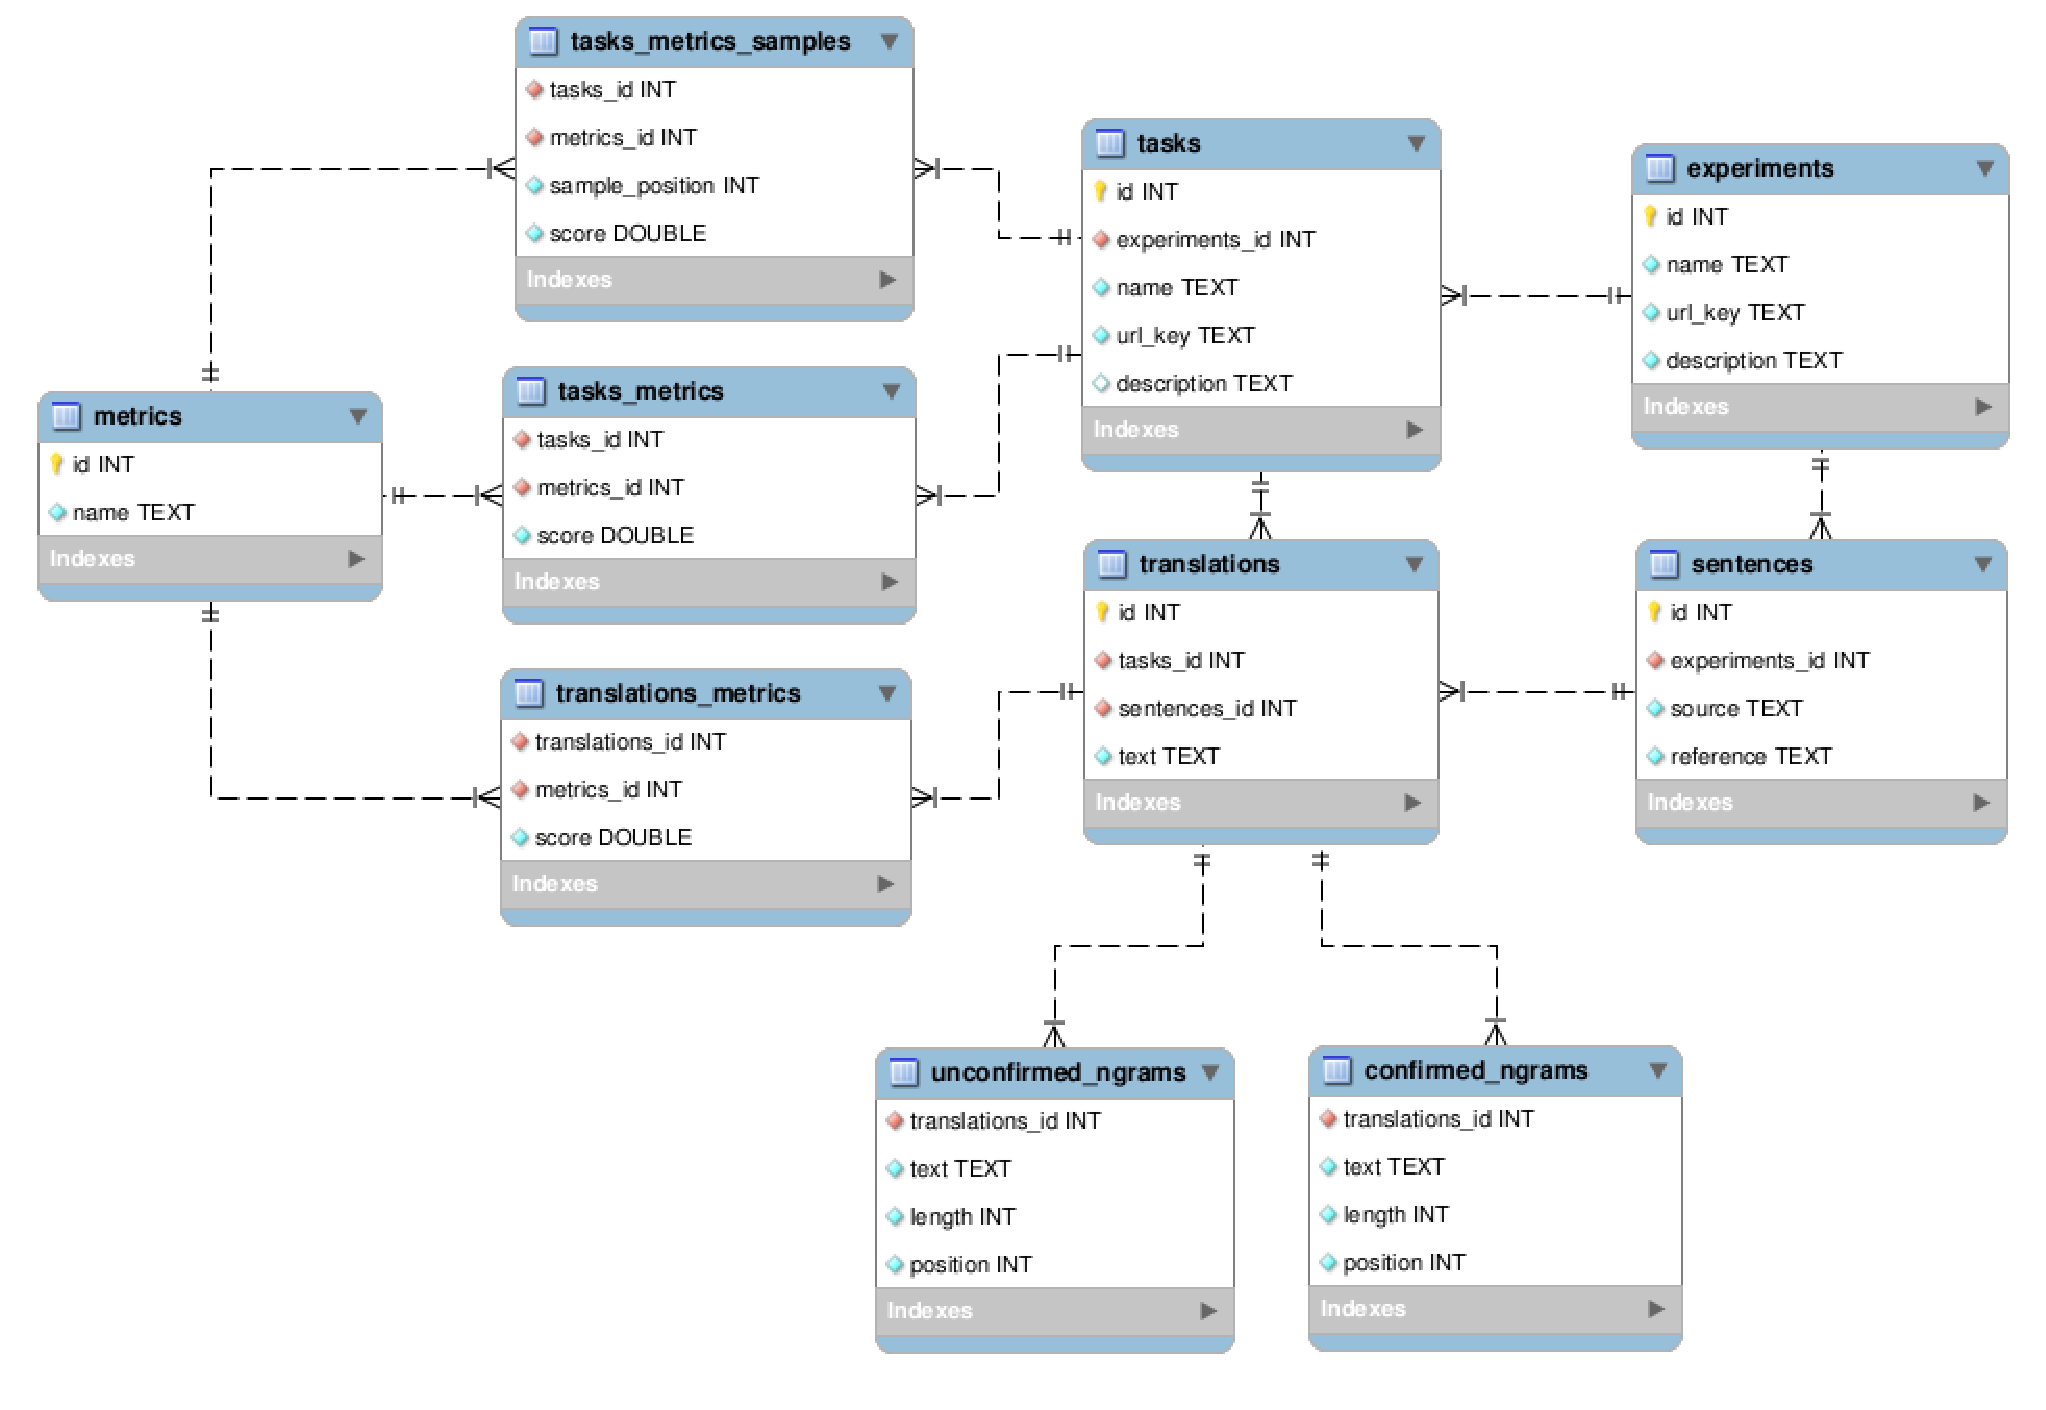
\includegraphics[width=0.8\textwidth]{img/schema.eps}}}
\section{Import experimentů a tásků}
\section{REST API}
\section{Frontend}

MT-ComparEval slouží k porovnávání a vyhodnocování strojových překladů.
Hlavním požadavkem při vývoji aplikace bylo,
  aby bylo možné jednoduše sputit aplikaci na vývojářově počítači.
Proto byly použity technologie,
  které jsou běžně dostupné na většině linuxových distribucí.
Jako hlavní programovací jazyk byl použit jazyk PHP ve verzi 5.4 
  s použitím frameworku Nette\footnote{http://www.nette.org}
  a jako databáze byla použita databáze SQLite3\footnote{http://www.sqlite.org}.
Jazyk PHP ve verzi 5.4 má v sobě obsažen jednoduchý webový server,
  tudíž je možné aplikaci bez větších obtíží spustit na vývojářově počítači.
V případě, že by měla aplikace běžet na serveru,
  je možné použít např. Apache HTTP Server.
Pokud by měla aplikace zpracovávat velké množství překladů,
  je možné použít i jiné databáze,
  ale bude potřeba přizpůsobit konfiguraci aplikace.
Na frontendu byl použit javascript s frameworkem AngularJS.\footnote{http://www.angularjs.com}


MT-ComparEval je webová aplikace skládající se ze tří částí:

\begin{itemize}
	\item serverové části pro import jednotlivých překladů
	\item serverové části pro vykreslování šablon a REST API
	\item frontendové části pro interaktivní porovnávání překladů
\end{itemize}

\section{Import překladů}
Aplikace MT-ComparEval byla navržena tak,
  aby ji bylo možné snadno zasadit do vývojového procesu strojových překladů.
Nepředpokládali jsme,
  že by si uživatel manuálně nahrával jednotlivé překlady k porovnání.
Spíše se předpokládá, že uživatel bude mít nastavený vývojový proces tak,
  že po každém úspěšném překladu se výsledný překlad nahraje do naší aplikace,
  kde si uživatel bude moci prohlédnout daný překlad v porovnání s ostatními překlady.

Vyhodnocování projektu probíhá proti referenčnímu překladu od překladatele.
Aby uživatelé mohli porovnávat své překladové systémy proti různým referenčním překladům,
  je možné si v naší aplikaci vytvořit různé uv{experimenty}. 

Experiment obsahuje zdrojový text, z kterého vznikaly překlady, a referenční překlad.
Každý experiment je uložen jako adresář,
  který obsahuje soubor se zdrojovým textem, referenčním překladem
  a konfigurační soubor.
V současné době aplikace umožňuje mít pouze jeden referenční překlad v experimentu,
  protože i ve většině soutěží se používá pouze jeden referenční překlad.

Do každého experimentu si může uživatel libovolně nahrávat nové strojové překlady.
V aplikaci tyto překlady nazývame uv{tasky}.
Každý task je uložen jako podadresář adresáře s experimentem
  a obsahuje soubor se strojovým překladem
  a konfigurační sobour. 

U všech souborů s překlady předpokládáme, že jsou zarovnané po větách.
Konfigurační soubory v obou případech slouží k přidání metainformací o experimentu/tasku,
  které mohou být později použity ve webové aplikaci.

\subsection{Import experimentů}
Všechny experimenty, které chceme naimportovat do naší aplikace,
  se musí uložit do adresáře \textbf{./data} v kořenu aplikace.
Nad tímto adresářem bdí proces, který hlídá,
  jestli zde nepřibyl nějaký nový experiment.
V případě, že objeví nějaký nový experiment,
  spustí další proces, který tento experiment naimportuje.

Při importu experimentu se nahrají všechny zdrojové věty
  a referenční překlady do databáze,
  abychom je mohli později použít při importu tasků
  nebo zobrazování výsledků.

Po úspěšném importu je do adresáře s experimentem přidán soubor,
  který nám označí daný experiment jako úspěšně naimportovaný.
Toho využijeme při importu tasků,
  abychom se nepokoušeli importovat tasky v experimentech,
  které ještě nebyly úspěšně naimportovány.
Zárověň tento zámek využijeme k tomu,
  abychom některý experiment nenaimportovali vícekrát.

%% TODO zamek pro neuspesne importy
Při importu experimentů může dojít k různým chybám -
  ať už na straně uživatele nebo na straně MT-ComparEval.
V případě, že nějaká chyba nastane,
  je do adresáře s experimentem přidán soubor,
  který nám označí,
  že při importu experimentu došlo k chybě
  a neměli bychom se ho pokoušet importovat znovu.
Když uživatel opraví chybu,
  která způsobila neúspěch importu,
  může tento soubor odstranit
  a MT-ComparEval se pokusí daný experiment znovu naimportovat.

\subsection{Import tasků}
Tasky, které chceme naimportovat do naší aplikace,
  se musí uložit do adresářů experimentů,
  ke kterým daný task patří.
Nad těmito adresáři bdí stejný proces
  jako proces pro import experimentů.
Tento proces hledá nový task ve všech již 
  naimportovaných experimentech.

Při importu tasku se nahrají všechny přeložené věty do databáze.
Zároveň musíme celý task vyhodnotit a předpočítat hodnoty,
  které později použijeme na frontendu.
Mezi tyto hodnoty patří:
\begin{itemize}
	\item metriky pro celý překlad a jednotlivé věty
	\item hodnoty pro Bootstrap Resampling 
	\item zlepšující/zhoršující n-gramy
\end{itemize}

\subsubsection{Předzpracování vět}
Jelikož se při importu tasků mnohé výpočty opakují
  ( počítání metrik, boostrap resampling, hledání společných n-gramů, \dots ),
  chceme si je předpočítat,
  abychom je mohli později použít a nemuseli je pokaždé počítat znovu.

Pokud chceme,
  aby naše výsledky výpočtu metrik byly stejné jako u jiných nástrojů,
  musíme text nejprve znormalizovat.
Znormalizování nám přidá mezery před a za všechna interpunkční znaménka.
Tím nám oddělí všechna slova a diakritiku - dále je budeme nazývat tokeny.
Znormalizovaný text můžeme tokenizovat (rozdělit na jednotlivá slova a diakritiku).
S takto získanými tokeny můžeme počítat libovolné metriky,
  aniž bychom se museli bát,
  že se naše výsledky budou lišit od výsledků jiných nástrojů.

Dalším krokem při předzpracování je získaní všech n-gramů z referenčního a strojového překladu.
N-gramem rozumíme posloupnout n po sobě jdoucích slov.
V nástroji MT-ComparEval počítáme pouze s n-gramy délky 1-4,
  tudíž při předzpracování hledáme pouze n-gramy těchto délek. 

Z n-gramů ze strojového překladu najdeme potvrzené n-gramy
  ( vyskytují se i mezi referenčními n-gramy )
  i n-gramy nepotvrzené.
Z těchto n-gramů později vypočítáme n-gramy,
  které nejvíce zlepšují/zhoršují skóre daného systému.
  
Jelikož při výpočtu BLEU nepotřebujeme znát jednotlivé n-gramy,
  z předpočítaných n-gramů si uložíme pouze jejich počty podle délky.
To nám ušetří mnoho času při výpočtu hodnot pro bootstrap resampling.

\subsubsection{Zpracování vět}
Hlavním cílem při zpracování vět je spočítat metriky jak pro jednotlivé věty,
  tak pro celé překlady.
Pomocí metrik u jednotlivých vět můžeme řadit věty tak,
  abychom zobrazili pouze věty, 
  které nás zajímají.
To jsou věty, u kterých došlo k největší změně.
%% vlozit screenshot s ukazkami vet
Pomocí metrik u celých překladů můžeme rozhodnout,
  který překlad je lepší
  nebo jestli se námi používaný překladový systém zlepšuje/zhoršuje.
%% vlozit ukazku vypisu tasku.

Metriky se počítají vždy v páru - case sensitive / case insensitive.
To proto, že se potvrzený n-gram může nacházet v referenčním překladu na začátku věty,
  kde bude začínat velkým písmenem,
  ale ve strojovém překladu se bude nacházet uprostřed věty,
  kde bude začínat malým písmenem.
%% vlozit ukazku vety, ktera zacina potvrzeným n-gramem.
Potom budou dávat obě metriky různé výsledky 
  a je jen na uživateli,
  aby si zvolil, která metrika ho více zajímá.

Aby si uživatel mohl doimplementovat další metriky,
  může TaskImporter použít libovolné množství implemantací rozhrani Metric.
Díky tomu je možné porovnávat výsledky pomocí různých metrik.

\subsubsection{Dokončení importu}
Před tím, než nahrajeme data do databáze, je nutné,
  abychom si dopočítali poslední informace,
  které potřebujeme ke správnému chodu frontendu,
  ale které jsou výpočetně náročné,
  tudíž by trvalo dlouhou dobu,
  než by je REST API spočítalo.

Mezi tyto informace patří vygenerovaní vzorků pro bootstrap resampling a
  nalezení nejvíce zlepšujících resp. nejvíce zhoršujících n-gramů.

\subsubsection{Bootstrap resampling}
%% rozsirit sekci o bootstrap resamplingu
Abychom mohli efektivně porovnávat dva překlady pomocí metody bootstrap resampling,
  musíme si předgenerovat velké množství náhodných vzorků.
My chceme,
  abychom vždy porovnávali stejné vzorky,
  ale abychom je nemuseli počítat při každém porovnávání počítat znovu.
Na začátku generování náhodných vzorků tedy nastavíme stejné jadérko generátoru náhodných čísel.
Tím dosáhneme toho,
  že všechny vzorky budou obsahovat vždy stejné věty
  a nemusíme tedy generovat vzorky pro všechny dvojice tasků v experimentu.
Náhodné vzorky počítáme pro všechny dostupné metriky,
  protože rozhraní pro výpočet jednotlivých metrik nám umožňuje spočítat danou metriku pro libovolnou testovací sadu,
  můžeme tyto výpočty znovu použít.


\subsubsection{Hledání nejvíce zlepšujících/zhoršujících n-gramů}
Nástroj MT-ComparEval nabízí i výpis nejvíce zlepšujících resp. nejvíce zhoršujících n-gramů.
Ty získáme tak, že vezmeme všechny potvrzené resp. nepotvrzené n-gramy
  a uděláme rozdíl obou porovnávaných překladů.
N-gramy,
  které mají největší rozdíl mezi jednotlivými překlady,
  jsou nejvíce zlepšující resp. nejvíce zhoršující.

Jelikož potvrzených resp. nepotvrzených n-gramů může být velké množství
  a nalezení nejvíce zlepšujících resp. nejvíce zhoršujících n-gramů může být pomalé,
  je potřeba,
  abychom našli všechny zlepšující resp. zhoršující n-gramy předem.
Při importu tasku tedy vezmeme všechny ostatní tasky z daného experimentu
  a pro ně předpočítáme 10 nejvíce zlepšujících resp. zhoršujících n-gramů. 

Abychom udělali počítání zlepšujících resp. zhoršujících n-gramů co nejefektivnější,
  používáme algoritmus podobný mergesortu,
  který z databáze postupně načítá n-gramy seřazené podle textu a věty, ve které se nacházejí, 
  a slévá je dohromady tak, že:

\begin{itemize}
  \item Pokud jsou oba n-gramy stejné, můžeme pokračovat ve výpočtu s další dvojicí.
    Pouze zaktualizujeme počet výskytů n-gramů v jednotlivých překladech. 
  \item Pokud se n-gramy liší, přidáme zlepšující resp. zhoršující n-gram k překladu,
    ve kterém se nachází uv{menší n-gram}. \\
    uv{Menší n-gram} je ten, který se nachází ve větě s nižším pořadovým číslem
    nebo je lexikograficky menší.
\end{itemize}

Na závěr vybereme 10 nejlepších resp. nejhorších n-gramů
  a uložíme si je pro pozdější použití.
Tímto alogirtmem dosáhneme lineární paměťové složitosti a
  lineární časové složitosti v závislosti na počtu potvrzených resp. nepotvrzených n-gramů.

%% TODO dodelat vypnuti predpocitani tasku
I přes to, že časová složitost předpočítání je lineární,
  může být předpočítání pro všechny ostatní tasky časově náročné
  (časová složitost je lineárně závislá na počtu tasků v experimentu),
  proto je možné toto předpočítání v konfiguraci jednotlivých tasků vypnout.
V porovnání dvou tasků pak nebudou předpočítané n-gramy k dispozici
  a je potřeba spustit skript,
  který je pro daný task zpětně dopočítá.

\subsubsection{Uložení předpočítaných dat do databáze}
Předpočítaná data pro jednotlivé tasky ukládáme do databáze SQLite3.
Při importu tasků chceme uložit velké množství dat,
  což by mohlo trvat velmi dlouho.
Proto jsou všechna data uložena v jedné transakci,
  která je mnohem rychlejší,
  než postupné ukládání.
Navíc tím získáme jistotu,
  že se nám do databáze nedostanou tasky,
  jejichž import se z různých důvodů nemusel povést.
 
\subsubsection{Logování importů}
%% přidat ukázky logů
Všechny důležité operace spojené s importem tasků či experimentů
  ( ať už je to načítání konfiguračního souboru, načítání vět ze souborů,
  počítání metrik, ukládání do databáze nebo některé další ), 
  jsou logovány do souboru,
  z kterého později můžeme vyčíst,
  proč nebyl některý task či experiment úspěšně naimportován. 


\section{REST API}
REST API je implementované v jazyce PHP s použitím frameworku Nette.
Slouží k předávání předpočítaných informací frontendu,
  který si je dle potřeby získává za použití AJAXu.
Api vždy vrací data ve formátu JSON,
  který můžeme snadno použít v javascriptu.
Pomocí api navíc můžeme získávat pouze data,
  která v danou chvíli potřebujeme.
Tzn. že nebudeme načítat všechny věty naráz,
  ale můžeme si je načítat postupně,
  s tím jak si je uživatel prohlíží.
Stejně tak nemusíme stahovat všechna data pro grafy,
  ale stačí nám stáhnout data pro právě vybranou metriku.

Pomocí api získáváme většinu dat pro porovnání dvou překladů,
  ať už jsou to dostupné metriky,
  data pro vykreslení grafů právě vybrané metriky,
  zlepšující resp. zhoršující n-gramy
  nebo věty,
  které můžeme řadit podle libovolné metriky a získavat je po částech.

V případě, že bychom chtěli zefektivnit použítí api tak,
  aby se všechna data musela počítat pouze jednou,
  můžeme použít reverse proxy cache - např. Varnish Cache.
To nám může výrazně ušetřit výpočetní výkon a zlepšit dobu odezvy api v případě,
  že aplikaci bude používat hodně uživatelů
  a bude v ní nahráno hodně experimentů/tasků.

\section{Frontend}
Na frontendu byl použit CSS framework Bootstrap od firmy Twitter,
  díky kterému bylo jednoduché vytvořit poměrně působivý design,
  a javascriptový framework AngularJS.
Jedná se o MVC framework vyvíjený ve firmě Google,
  mezi jehož hlavní přednosti patří 2-way data binding -
  tzn. že při změně v modelu nebo nějaké uživatelské interakci se stránky automaticky překreslí.
Díky tomu je možné deklarativně popsat chování stránek,
  které pak si při každé uživatelské akci stáhnou potřebná data z api
  a není tak potřeba psát kód pro různé situace.

Na frontendu se nacházejí tři typy stránek:
\begin{itemize}
  \item seznam všech experimentů
  \item seznam všech tasků v daném experimentu
  \item porovnání dvou tasků
\end{itemize}

Seznamy experimentů a tasků slouží pouze k výběru tasků,
  které chceme porovnávat,
  proto se jedná pouze o výpis jmen s upřesňujícími informacemi.

%% TODO přidat graf vývoje 
V seznamu tasků daného experimentů navíc můžeme vidět graf s vývojem jednotlivých metrik tasků.
Pomocí něho si můžeme rychle udělat přehled,
  jak se překlady zlepšují resp. zhoršují.
Pokud by nám informace z grafu nestačily,
  je možné najít přesné hodnoty metrik v tabulkách u jednotlivých tasků.
Na základě těchto informací si můžeme vybrat,
  které tasky má smysl porovnávat.
Díky jednoduchému procházení experimentů a tasku se můžeme zaměřit na nejdůležitější část aplikace
  - porovnávání dvou tasků.

Dva tasky můžeme porovnávat na základě několika kritérií,
  kterým odpovídá záložka na stránce s porovnáním dvou tasků:
%% TODO přidat obrázek s výběrem záložek
\begin{itemize}
  \item Sentences - porovnání na základě překladu jednotlivých vět
  \item Statistics - porovnání na základě výsledků jednotlivých metrik
  \item Confirmed n-grams - porovnání na základě nejvíce zlepšujících n-gramů
  \item Unconfirmed n-grams - porovnání na základě nejvíce zhoršujících n-gramů
\end{itemize}

Abychom nemuseli složitě přecházet mezi stránkami,
  když chceme porovnávat jiné tasky z experimentu,
  je možné měnit tasky přímo v porovnání.


\subsubsection{Porovnání na základě překladu jednotlivých vět}
Při porovnávání dvou překladů nás nejvíce zajímají věty,
  které se nejvíce zlepšily resp. zhoršily.
To poznáme tak, že se rozdíl metrik nejvíce liší. 
Proto jsou věty vždy seřazeny podle rozdílů metrik.
Metriky můžeme libovolně měnit a stránka se automaticky zaktualizuje.
Zároveň se změnou metriky můžeme ovlivnit,
  v jakém pořadí budou věty načítány.
Tím můžeme určit,
  jestli nás zajímají věty,
  které se nejvíce zlepšily resp. zhoršily.
Jelikož načtení všech vět by mohlo být náročné,
  načítají se vždy věty s tím,
  jak se uživatel postupně posouvá stránkou.
Často nám stačí prohlédnout pouze několik vět,
  abychom si udělali obrázek,
  v čem se dva porovnávané tasky nejvíce liší.
Aby si mohl uživatel vybrat,
  které překlady ho zajímají,
  může si skrýt a zobrazit zdrojovou větu, referenční překlad nebo porovnávané překlady.
Toho může využít, když ho zajímá např. pouze porovnání jednoho překladu s referencí a
  ostátní překlady by ho mohly rušit.

%% vložit obrázky s porovnáváním vět a zvýrazněnými potvrzenými, zlepšujícími nebo zhoršujícími n-gramy
Aby uživatel mohl snáz porovnávat překlady vět,
  může si dle chuti zapnout / vypnout zvýraznění všech potvrzených n-gramů,
  zlepšujících n-gramů nebo zhoršujících n-gramů.
Za zlepšující n-gramy jsou považovány ty potvrzené n-gramy,
  které se nacházejí pouze v jednom z porovnávaných překladů.
To stejné platí pro zhoršující n-gramy,
  které ale vybíráme z nepotvrzených n-gramů.
Na základě barevného podbarvení jednotlivých slov pak uživatel může poznat,
  která slova jsou přeložena lépe či hůře.

Další možností jak rychle porovnat překlady je zvýraznit diff mezi překladem a referenčním překladem.
Ve většině případů se toto zvýraznění nebude odlišovat od zvýraznění potvrzených n-gramů -
  zvýrazněné potvrzené n-gramy se nacházejí jak v referenčním tak v porovnávaném překladu
  a nezvýrazněná slova se nenacházejí v jednom z překladů.
Jediný rozdíl mezi těmito zvýrazněními nastane,
  když se bude lišit slovosled porovnávaných překladů,
  pak může být povrzený n-gram označen za chybějicí resp. přebývající.

\subsubsection{Porovnání na základě výsledků jednotlivých metrik}
%% vlozit obrazek s porovnáním vysledku dvou tasku
Rychlý přehled o kvalitě jednotlivých překladů si můžeme udělat pohledem na výsledky jednotlivých metrik.
Ať už se jedná o data v tabulce s metrikami nebo graf hodnot jednotlivých metrik,
  graf rozdílů aktuální metriky u vět nebo graf bootstrap resamplingu.
Grafy se automaticky překreslují při změně metriky,
  podle které se mají řadit věty,
  tím si může uživatel zobrazit grafy pro všechny nabízené metriky.


\subsubsection{Porovnání na základě nejvíce zlepšujících resp. zhoršujících n-gramů}
%% vlozit obrázek s výpisem nejvíce zlepšujících / zhoršujících n-gramů
Dobrý obrázek o zlepšení / zhoršení překladu si můžeme udělat,
  když se podíváme,
  v kterých n-gramech se dané překlady nejvíce liší,
  ať už se jedná o zlepšující n-gramy nebo n-gramy zhoršující.
Nástroj MT-ComparEval vypisuje seznam zlepšujících resp. zhoršujících n-gramů seskupených podle délky,
  pomocí něhož můžeme filtrovat věty a prohlížet si pouze ty,
  v kterých se daný zlepšující resp. zhoršující n-gram nachází.
Vybraný n-gram je následně ve všech větách zvýrazněn,
  aby uživatel mohl rychle zjistit, kde se nachází -
  může se totiž stát, že se daný n-gram ve větě bude nacházet vícekrát,
  ale pouze některý z nich bude zlepšující resp. zhoršující.

Jelikož se daný n-gram může nacházet v mnoha větách,
  nenačítáme všechny věty naráz,
  ale věty jsou načítány postupně,
  stejně jako když procházíme věty v normálním režimu.
Stejně tak se může stát,
  že se v jedné větě vyskytne zlepšující n-gram vícekrát
  ( typicky se to stává u interpunkce, spojek nebo předložek ),
  tyto věty nás zajímají více než věty,
  ve kterých je výskytů daného n-gramu méně.
Proto jsou věty při filtrování podle zlepšujícího resp. zhoršujícího n-gramu vždy řazeny podle počtu výskytů daného n-gramu ve větě
  a nejde je řadit podle rozdílu metrik jako v normálním módu.

%% vlozit obrazek zhorsujiciho n-gramu, ktery obsahuje zlepsujici n-gram
Při zobrazování delších zhoršujících n-gramů může nastat situace,
  že si uživatel nechá zvýraznit všechny zhoršující n-gramy,
  ale vybraný zhoršující n-gram nebude zvýrazněn.
Dokonce se může stát, 
  že si uživatel nechá zvýraznit všechny potvrzené n-gramy
  a část vybraného zhoršujícího n-gramu bude zvýrazněna.
Toto je úplně normální jev,
  který je způsoben výběrem potvrzených n-gramů,
  je jedno, kde se daný potvrzený n-gram nachází,
  stačí,
  že se někde ve větě objeví a už je prohlášen za potvrzený.
Změnou slovosledu pak může dojít i k situaci,
  kdy se zhoršující n-gram velké délky bude skládat z potvrzených n-gramů délky kratší,
  které se nacházely na různých pozicích ve větě. 
Například stačí, aby byly ve správném pořadí,
  ale bylo mezi nimi vypuštěno alespoň jedno slovo.
Proto je lepší,
  aby uživatel porovnával překlady spíše podle n-gramů s menší délkou -
  typicky podle 1-gramů a 2-gramů.
Aby mělo smysl porovnávat překlady podle delších n-gramů,
  musel by být překladač otestován na velké počtu vět tak,
  aby se zlepšení resp. zhoršení dostatečně projevilo.

\section{Zobrazení potvrzených n-gramů a diffu pomocí}
Pro správné zobrazení potvrzených n-gramů a diffu je potřeba,
  abychom mohli každému tokenu říci,
  jestli se nachází v nějakém potvrzeném n-gramu nebo jestli byl do věty přidán.
Zároveň s touto informací chceme,
  aby jednotlivá zvýraznění bylo možné libovolně kombinovat.
Technicky tento problém byl vyřešen pomoci CSS tříd,
  kdy každému tokenu byly přiřazeny třídy v závislosti na informacích,
  které jsme si vypočítali pomocí výše uvedených postupů.
Zapnutí a vypnutí jednotlivých kombinací je pak otázkou přiřazení příslušné třídy kořenovému elementu,
  v kterém se nacházejí všechny věty.
Přehlednost těchto kombinací nemusí být vždy zcela ideální, 
  proto jsme se snažili udělat jednotlivá zvýraznění tak,
  aby byla co nejjednodušeji modifikovatelná.
Každý typ zvýraznění tak má vlastní selektor,
  pomocí kterého může zvýraznění v CSS upravit.

